%%%%%%%%%%%%%%%%%%%%%%%%%%%%%%%%%%%%%%%%%
% Stylish Article
% LaTeX Template
% Version 2.0 (13/4/14)
%
% This template has been downloaded from:
% http://www.LaTeXTemplates.com
%
% Original author:
% Mathias Legrand (legrand.mathias@gmail.com)
%
% License:
% CC BY-NC-SA 3.0 (http://creativecommons.org/licenses/by-nc-sa/3.0/)
%
%%%%%%%%%%%%%%%%%%%%%%%%%%%%%%%%%%%%%%%%%

%----------------------------------------------------------------------------------------
%	PACKAGES AND OTHER DOCUMENT CONFIGURATIONS
%----------------------------------------------------------------------------------------

\documentclass[fleqn,10pt]{SelfArx} % Document font size and equations flushed left


%----------------------------------------------------------------------------------------
%	Source Code Listings
%----------------------------------------------------------------------------------------
\usepackage{listings}
\usepackage{xcolor}
\definecolor{darkgreen}{rgb}{0.0, 0.2, 0.13}
\definecolor{ao}{rgb}{0.0, 0.5, 0.0}
\lstdefinestyle{sharpc}{language=[Sharp]C, frame=single}
\lstset{% general command to set parameter(s)
basicstyle=\small, % print whole listing small
keywordstyle=\color{blue}\bfseries,
% underlined bold black keywords
commentstyle=\small\color{ao}, % white comments
stringstyle=\ttfamily, % typewriter type for strings
columns=fullflexible, % keeps the comments from exploding
showstringspaces=false} % no special string spaces


% Algorithms package
\usepackage{fancybox}
\usepackage{algorithm}
\usepackage{caption}
\usepackage{algorithmic}
\usepackage{bm}

\usepackage{breqn}

%----------------------------------------------------------------------------------------
%	COLUMNS
%----------------------------------------------------------------------------------------

\setlength{\columnsep}{0.55cm} % Distance between the two columns of text
\setlength{\fboxrule}{0.75pt} % Width of the border around the abstract

%----------------------------------------------------------------------------------------
%	COLORS
%----------------------------------------------------------------------------------------

\definecolor{color1}{RGB}{0,0,90} % Color of the article title and sections
\definecolor{color2}{RGB}{0,20,20} % Color of the boxes behind the abstract and headings

%----------------------------------------------------------------------------------------
%	HYPERLINKS
%----------------------------------------------------------------------------------------

\usepackage{hyperref} % Required for hyperlinks
\hypersetup{hidelinks,colorlinks,breaklinks=true,urlcolor=color2,citecolor=color1,linkcolor=color1,bookmarksopen=false,pdftitle={Title},pdfauthor={Author}}

%----------------------------------------------------------------------------------------
%	ARTICLE INFORMATION
%----------------------------------------------------------------------------------------

\JournalInfo{PBEP \#3, 2015} % Journal information
\Archive{PBEP Series} % Additional notes (e.g. copyright, DOI, review/research article)

\PaperTitle{PacBio Enhancement Proposal \#3 \\{\large Implementing a probability based scoring model for CCS}} % Article title

\Authors{Nigel Delaney and David Alexander} % Authors

\Keywords{} % Keywords - if you don't want any simply remove all the text between the curly brackets
\newcommand{\keywordname}{Keywords} % Defines the keywords heading name

%----------------------------------------------------------------------------------------
%	ABSTRACT
%----------------------------------------------------------------------------------------

\Abstract{ 
\\
The current PacBio CCS scoring model does not work in probability space, resulting in several oddities and inefficiencies.  This proposal presents a new scoring scheme that, conditioned on features associated with a read (such as QV scores) calculates the probability that the read could have generated the derived template by integrating over all possible paths of insertions, deletions, mismatches and matches between the read and the template. The probability model proposed is a combination of two standard statistical tools, namely conditional random fields and generalized linear models, and so greatly benefits from established theory and methods.  The use of this model would allow PacBio to rid itself of several disparate steps currently used in the consensus algorithms, including GBM modeling and hard-coded constants to establish QV scores, inefficient and biased methods to retrain these values for CCS, and the ad-hoc methods used following CCS to establish predicted accuracy.  Finally, using this model allows for a direct correspondence and shared code base between the parameters optimized by SMS (Edna) and those used in generating accurate reads from sequencing reactions.  \\


Statisticians -- for all the right reasons -- love unified models.  This is that model. }

%----------------------------------------------------------------------------------------

\begin{document}

\flushbottom % Makes all text pages the same height

\maketitle % Print the title and abstract box

\tableofcontents % Print the contents section

\thispagestyle{empty} % Removes page numbering from the first page

%----------------------------------------------------------------------------------------
%	ARTICLE CONTENTS
%----------------------------------------------------------------------------------------

\section{Introduction} % The \section*{} command stops section numbering


There is a long standing tradition in bioinformatics of generating alignments between sequences according to a dynamic programming method that scores alignments according to a fixed set of parameters for insertions, deletions, mismatches and matches.  More sophisticated frameworks treat the alignment problem using a probabilistic modeling framework, such as a Paired HMM model, in which there is a defined generative model with transition probabilities between insertion, deletion and match states.  It has been shown that when considering the optimal alignment, there is a direct correspondence, in math but not in intuition, between the probabilistic framework and the standard affine scoring dynamic programming method.\footnote{See the section \textit{The most probable path is the optimal FSA alignment} on page 82 in the book \textit{Biological Sequence Analysis} by Durbin et. al}

Using a probabilistic framework has numerous advantages compared to using a fixed scoring scheme.  Questions such as how much evidence is there for one alignment as compared to another are directly answered by comparing probabilities.  Additionally all the tools and historical research concerning probabilistic modeling become available, guiding the choices of model selection, optimization methods and offering asymptotic guarantees about their accuracy and bias.  Finally, in the context of DNA sequencing, probabilistic frameworks allow us to naturally integrate over all the ways a particular read could be generated from a particular template.

The PacBio analysis which generates consensus sequences does not currently use a probabilistic framework, a possibly glaring omission since there is a left-right generative HMM believed to govern how PacBio reads are created.  The central reason for this is that most probabilistic models use fixed parameters for transitions between states, while in practice there are often covariates associated with the bases of an emitted read that indicate how much certainty we have that they are a true representation of the template.

These covariates, typically condensed into QV values, are not easily incorporated into the PacBio probabilistic framework for how reads are generated, and so the statistical method of estimating models and parameters is abandoned in favor of a scoring scheme that rhymes with, though does not actually represent, a probability model.  The central difficulty of QV values is that they are properties of the \textit{read bases} rather than properties of the \textit{template} bases.  In the left-right generative HMM for PacBio data, the model transitions between states are governed by the template, which is the true fixed parameter from which the noisy sequence of reads is recovered.  In contrast, QV values only really make sense if the read is the generative model for the noisy template.  In particular, consider calculating the probability of a template given a read and quality scores, jointly denoted by $R$, using the standard Bayes corrollary.

\begin{dmath}
P(T|R) = \frac{P(R|T) \cdot P(T)}{P(R)}
\end{dmath}

Of the three quantities required by the right hand side of equation 1, two are unnecessary when finding the optimum template for $P(T|R)$.  The denominator, $P(R)$, is a common for all templates and so is uninformative when making comparisons between them. $P(T)$, although seemingly essential, can typically be set to some uninformative (or uniform) prior and so can similarly be avoided.  However, although our generative Edna model can in theory provide a mechanistic way to calculate the sequence observed in the read data, $R$, there is no generative model for the QV values of $R$ and as a result the essentially needed and remaining quantity $P(R|T)$ cannot be calculated.

A possible path forward that would still allow us to use QV values to capture local uncertainty in sections of the reads is to invert the generative model.  That is rather than have a model, like Edna, which generates $R|T$, we envision a left right HMM that generates $T|R$.  By undertaking this reversal of the generative process, we can naturally incorporate QV values as they are once again properties of the `template', rather than of the observed data.  Template selection is then simply a matter of finding $T$ such that we maximize $P(T|R)$.  If the model is calibrated correctly, we can still express our confidence for a given template or variants of it by comparing values of $P(T|R)$.

Although reversing the generative process in this way allows for a natural incorporation of QV values, it also completely inverts the inference process, to the point where we could really be said to be doing probabilistic modeling rather than statistical inference.  In fact, this is exactly what we are doing.  While in the original $P(R|T)$ framework we would use the observed data to calculate the probability of an unknown underlying parameter, $T$, in the new framework we are using known values, the $R$, which are essentially fixed parameters, to calculate the probability of producing data we never observe, $T$.  We are looking for the most probable outcome rather than parameters that best explain the data.

Although this may initially seem like a strange path, we'll show that there is a natural correspondence between the generative models used for $P(R|T)$ and $P(T|R)$, with the later being a mirror image of the former.  Therefore, although the reality is not that templates are generated from reads, we should expect that this statistical model should very well approximate the reality, in much the same way logistic regression might approximate a binomial outcome, despite rarely representing a physical process.

This proposal attempts to create a framework for PacBio consensus scoring that represents a true probability model according to the $P(T|R)$ framework.  It will do this by making the central conceit already mentioned, which is to invert the relationship between the read and the template so that we maximize the likelihood of templates being emitted by reads.

The model proposed for $P(T|R)$ is a left-right generative HMM that is designed to mirror the original generative model for PacBio data, thus approximating its mechanics.  For example, while the original generative model has a `merge` transition which represents the probability that two bases are emitted as one (a homopolymer deletion), the new generative model has a `spit` probability that represents the transition where a base is emitted twice (a homopolymer insertion).  In this way there is a direct correspondence between the `Edna` model and this new probability model.  Given this framework, we can then assess the total probability for $P(T|R)$ by integrating over all paths through the left-right HMM given by the read that would emit the specified template sequence.  The key feature that this model is able to exploit is that the transition between the read bases in the underlying left-right HMM are governed by the QV values that accompany each read base, allowing for them to naturally be accommodated in a generative and probablistic framework.  

I now review the original generative mode (Edna), and then explain the scoring model.


\section{The Model for $P(R|T)$}

PacBio emits reads when sequencing a given template and our probabilistic model for this is motivated by our biological understanding of the sequencing process.  This section attempts to explain both the model and the reality it is designed to approximate.

In PacBio sequencing, the enzyme traverses along the template and as it incorporates nucleotides connected to fluorescent molecules, this creates 'pulses' detected by our optical equipment which are converted into basecalls.\footnote{https://www.youtube.com/watch?v=NHCJ8PtYCFc}  Our current model envisions 5 separate processes that can occur as a basepair is being incorporated by a template:


\begin{enumerate}
  \item \textbf{A Correct Emission (Match)} - The basepair is acquired by the enzyme, and a single fluorescent pulse is detected.  Typically, this pulse is identifed as coming from the corresponding fluorophore of the incorporated basepair, but occasionally may be miscalled due to an instrumentation error, which creates a substitution when viewed by later alignments.
  \item \textbf{A Missed Emission (Deletion)} - Sometimes the fluorescent signal emitted during nucleotide incorporation is not enough to meet the criteria to be emitted as a space, leading to a base which was actually incorporated not causing a basepair to be emitted.
  
    \item \textbf{A Merge (Deletion) } - Occasionally, the enzyme will incorporate two basepairs that are only detected as one pulse.  This can occur if either the distance between acquiring separate molecules is too short to be detected, or if the   
   
  
  \item \textbf{A Failed Incorporation (Insertion) } - Occasionally, the enzyme will begin to incorporate a base, but release the bound nucleotide before finishing the incorporation reaction.  This is often referred to as a branch and results in the emission of the same basepair as the true basepair which is next incorporated.
  
  \item \textbf{A Stick (Insertion) } - Sometimes, either the instrument `hiccups' and emits pure noise as a pulse equivalent to a basepair or a fluorescent molecule will randomly float into the detection level of the ZMW and will appear as a signal despite not being connected to an incorporation reaction (this behavior of `sticking' to the bottom of the ZMW leads to the given name).  Although one might think of this event leading to any basepair with equal probability, fluorphores may be quite biased to emit certain basepairs.
     
\end{enumerate}


Although additional complexity may be at play, and if believed to be important should be accounted for, at present these are the dominant processes believed to occur as the PacBio technology converts basepairs into reads and so for the basis of the approximating HMM model described next.

\begin{figure*}[ht] %% The [h] means place the figure about here.
	\frame{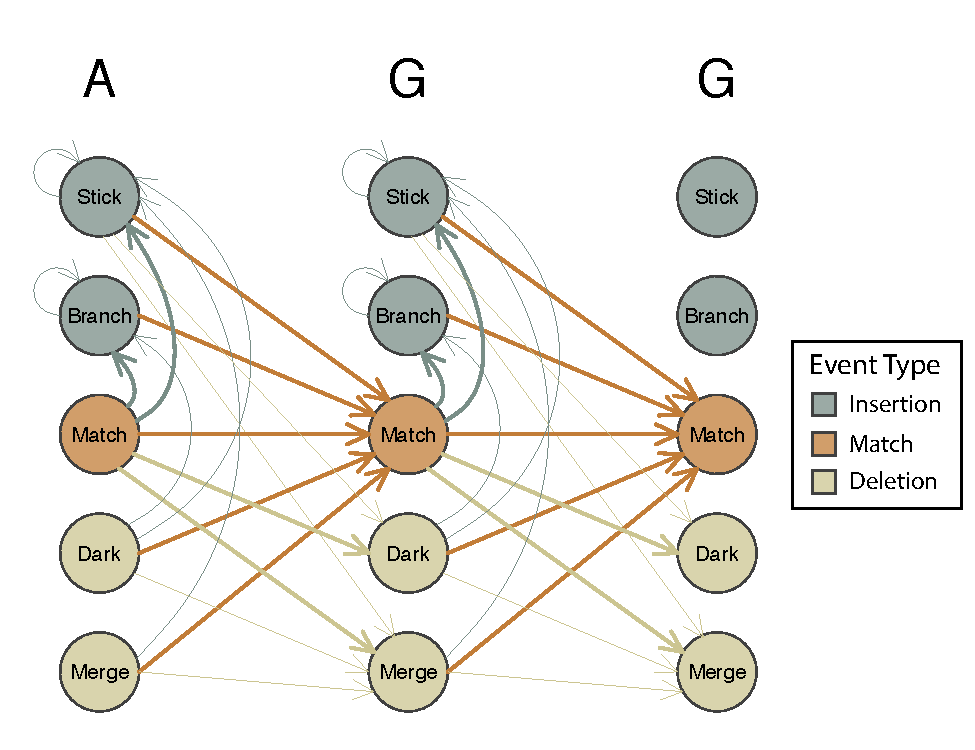
\includegraphics[width=\linewidth]{Hmm}}
		\caption{The left-right HMM that defines the paths by which an example template (AGG) can produce reads.  Each circle represents a latent state that can produce basepairs (or no observation for nodes colored as deletions) if visited by a stochastic path through the HMM.  Possible transitions into and out of each read are indicated by arrows.  Thick arrows represent paths presumed to be the most frequently used, while thin arrows represent less common occurrences. }				
\end{figure*}

\subsection{The Left to Right HMM}
An HMM model is defined by a structure which defines what symbols are emitted and how latent states connect, as well as a set of transition probabilities across those connections, $\Lambda$, a set of emission probabilities for possible observations, $\epsilon$, and a probability distribution for the initial state, $\pi$.   We will refer jointly to the parameters of the model as $\theta = [\Lambda, \epsilon, \pi]$.


Figure 1 shows the structure of the HMM that determines how a template would emit reads when sequenced by the RS.  Not shown are the emission probabilities, but these follow directly from the mechanisms enumerated above.  For example, in a deletion event no basepair is emitted, while in a stick a random basepair is emitted, and in a branch the basepair matching the next template position is emitted (with some probability of miscalls for all emissions).   

Importantly, this HMM structure is identical to a conditional random field, or CRF model, and so we can use all the standard tricks that apply to such models.  For example, in order to calculate the likelihood of a given read being emitted from a template, we can use the standard dynamic programming methods.  In this framework, each class of latent variable is represented by a position in an $ M \times N$ matrix which stores the probability that for the emission $i$ we were at template position $j$ and at the type of node stored by the matrix (as shown in Figure 2).  We then recursively populate each of these matrices using the standard algorithm described below.

\begin{algorithm}
\caption*{\textbf{Standard Recursion Algorithm to Calculate Probability }}
\label{calcScore}
\begin{algorithmic}[h]
\FOR{$j=1$ to J}
\FOR{$i=1$ to I}
\IF{ $i =0\ \& j =0 $}
\STATE $A[i,j] \leftarrow 0$
\ELSE
\STATE \[
	A[i,j]  \leftarrow \sum\nolimits_{\text{ All Connecting Nodes} } p_{\text{At Node}} \cdot p_{\text{Transistion}} \cdot p_{\text{Emission}}
	\]
\ENDIF	
\ENDFOR
\ENDFOR
\RETURN $A[I,J]$
\end{algorithmic}
\end{algorithm}



Although storing such large matrices for many reads may seem inefficient, in practice we can usually use a "reduced" model which allows us to store the values for multiple matrices in one.  In particular, if the possible transitions and probability for those transitions is identical for any set of node types, then the two matrices which store information for those node types can be combined into one (as  $p_{i \rightarrow j} \cdot p_{A} + p_{i \rightarrow j} \cdot p_{B} = p_{i \rightarrow j} (p_{A} + p_{B})  $ ).  In the extreme case where all such transitions probabilities are shared across node types, only one matrix is required for the recursion.

\begin{figure} %% The [h] means place the figure about here.
	\frame{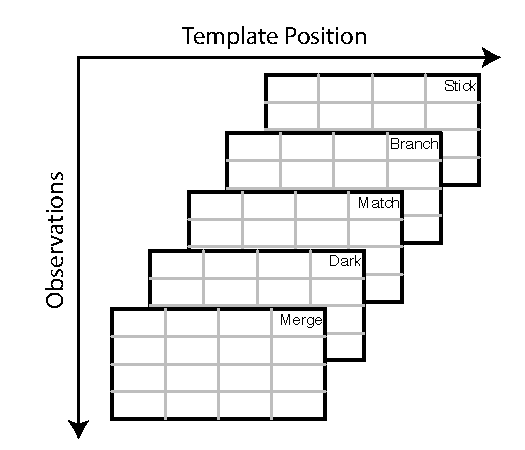
\includegraphics[width=\linewidth]{matrices}}
		\caption{The five matrices required in a full model to perform dynamic programming to calculate the likelihood in a full model specified by figure 1. }				
\end{figure}


While there are certainly trade-offs in model complexity versus computational speed, now that we have a probabilistic model we can use standard tools to intelligently evaluate those tradeoffs.  For example, we could assess the importance of a merge to merge transition, as opposed to a simpler model which sets this probability to 0, by comparing the AIC scores of a model with and without this parameter.

Inevitably evaluating this trade-off will be important, as the full model shown in figure 1 for each template position has 18 transition parameters for 5 latent nodes which implies that there are $18-5 = 13$ free transition parameters at each template position.  If we use a model which uses a different transition probability for each basepair type, this would require us to estimate $4 \times 13 = 52$ parameters parameters which govern the dynamics of stochastic paths through the CRF.  Fortunately, fitting and evaluating such models is straightforward, as the Baum-Welch algorithm allows for efficient estimation of the parameters in this model, and as stated the recursion allows us to quickly calculate the likelihood.

This CRF is a complete specification of the PacBio generative model, and the inference of the parameters in it is equivalent to finding the values produced by Edna.  As such, it can completely replace Edna.

%------------------------------------------------

\section{The New Scoring Model for $P(T|R)$ }

Given reads, if we want to estimate the probability for a template, we simply invert their relationship.  Seen from the perspective of the recursion matrices, this is exactly equivalent to "flipping" the placement along the axis so that the read bases now run along the top of the matrix and the template base run down the side.  As such, the same model as shown in figure 1 can be used, with the only change being that the labels and respective emission probabilities for insertion and deletion events are switched.  Fortunately, there is a direct correspondence between the types of deletions and insertions, with a Branch being equivalent to a Merge, and a Stick being equivalent to a Dark.  Therefore, while in our inverted framework what was previously seen as a deletion becomes an insertion, there is no need to write a separate scoring or optimization method.  The same CRF model and code base can be used for both, and the parameter estimates obtained from Edna can directly be used for the inverted inference process of $P(T|R)$.

The one critical difference though is that with read bases, we have features attached to them, covariates such as SNR, IPD, etc. that we may wish to incorporate into our scoring scheme.  A straightforward way to do this is to model the transition probabilities as functions of these variables, and to do this we can simply co-opt the tools of nominal logistic regression.

The central insight here is that in the CRF model shown in figure 1, picking a random path out of any node in the CRF is equivalent of making a draw of size 1 from a multinomial distribution.  Nominal logistic regression is the standard and well established way to model how certain covariates affect such outcomes, and we can therefore consider the problem of fitting transition probabilities as exactly equivalent to fitting the probabilities in a multinomial distributions as a function of these covariates.  As a quick review, in nominal logistic regression, the transition probability for one category, $\pi_{1}$, is arbitrarily set as the reference and the relative probabilities of the other transiitons are fit as linear functions of the covariates. \footnote{See \textit{An Introduction to Generalized Linear Models} by Dobson and Barnett or any other text on GLMs for a more complete explanation.}

\begin{dmath}
\text{logit} (\pi_{J}) = \text{log} ( \frac{\pi_{J}}{\pi_{1}}) = X \beta
\end{dmath}

In the machine learning field this is often referred to as a `softmax' function.  We can now consider the calibration of QV scores as equivalent to finding the parameters $\beta$ which are best fit for this model.  Once this model is fit, we then have a choice.  We can either directly emit the covariates, or features, that are used in the model from primary, or use the model to calculate the respective probabilities in primary and emit them as QV scores which directly represent different transition probabilities.  An example of how such QVs would be interpreted is shown in Table 1.  

\begin{table*}[bt]
\caption{Table of QV Meanings}
\centering
    \begin{tabular}{| l | p{7cm} | c |  }
    \toprule
    \hline
    \textbf{QV Value} &  \textbf{Represents the transition probability of:} &   \textbf{Analogous Edna State}  \\ \hline \hline
    Insertion Different & Match $\rightarrow$ Stick.  An insertion prior to this base of a different base than itself. &  Dark / null \\ \hline
    Insertion Same & Match $\rightarrow$ Branch. An insertion prior to this base of the same base as itself.&  Merge \\ \hline
    Deletion Different & Match $\rightarrow$ Stick. A deletion prior to this base of a different base than itself. &  Stick \\ \hline
    Deletion Same & Match $\rightarrow$ Merge. A deletion prior to this base of the same base as itself. &  Branch \\ \hline
    Substitution & Misclassified Match. This base being emitted correctly conditioned on it being emitted &   Misclassified \\ \hline
    \bottomrule
    \end{tabular}
\end{table*}

Note that as before, now that we have a unified statistical model, we can use all the statistical tools that come along with it.  For example, to examine which covariates affect the different error rates, and which features are necessary, we can simply compared models using standard tools such as AIC, deviance values or the Wald test to assess the importance of individual parameters.  The unified statistical model enables all of this.

\section{Model Training}

As the model specified here meets the criteria for the Cramer-Rao lower bound, maximum likelihood is the best choice for parameter estimation.  Although the model is more complicated, there is an immediate analogy to Baum-Welch which I believe makes EM a clear choice for fitting the model parameters, $\beta$.

The central intuition behind Baum-Welch is that given a set of observations from a multinomial distribution, estimating the parameters for a constant value probability model is trivial as the MLE for each emission parameter is:

\begin{dmath}
p = \frac{\text{ Times happened}}{\text{ Times could have happened}}
\end{dmath}

However, in the CRF model we never actually observe draws from the multinomial distribution, as the underlying path taken through the model is hidden.  As a result, one cannot apply this simple formula.  The EM algorithm allows a solution to this dilemma. 

which is an EM algorithm, in the E step one uses a current parameter guess to generate `pseudo-counts`, and then in the M step uses a slight modification of the above simple formula above to maximize the parameters, iterating until convergence.

A simple extension of this principle allows us to fit our model for $P(T|R)$ in the presence of covariates.  In nominal logistic regression the multinomial parameters are not fixed and so to find the MLE one cannot use the analytical solution as in the constant value case but must instead solve a non-linear optimization.  However, Fisher Scoring provides an efficient means to do this, and can often converge quite quickly.  Therefore, just as in Baum-Welch we use the current parameters of the model to generate pseudo-counts in the E step, in the M step we can simply use the standard nominal regression Fisher Scoring algorithm to maximize the parameters, again iterating until convergence. 


In doing so we will treat the read and it's associate QV values as fixed parameters, and given several such reads will find the template with the highest probability of occurring across a set of reads.  Although counterintuitive, once framed this way, we are easily able to incorporate the probabilities given by QV values and work in a probabilistic way.  This framework also allows us to cleanly separate the domains of primary and secondary analysis, with the transition between the two demarcated by the paradigm shift  $P(R|T) \rightarrow P(T|R) $ and the concurrent generation of the respective QV values as probabilities of certain events (which can be framed as maximizing the fixed parameters given the observed template). 




\begin{figure*}[h] %% The [h] means place the figure about here.
	\frame{\includegraphics[width=\linewidth]{OldvNewFigure}}
		\caption{A comparison of the set of inter-related components required for the older as compared to the newer framework.  Boxes represent separately maintained models and code bases, and arrows indicated dependencies between modules. }				
\end{figure*}


\subsection{ Calculating $\mathbf{P(T|R)}$} 

The inputs are a read of length, J, and a template of length I.  Each base in the read also has an associated QV values given by Table 1.   The algorithm proceeds by recursively populating a matrix and returning the bottom right value as described next.  In describing the algorithm and to account for offsetting, in what follows read and template positions are 1-based indexed, while positions in the matrix that are filled are referred to by 0-based indexes. 






\subsection{Recursion steps}
After the matrix is initialized, each element in the matrix is recursively populated with the logarithm of the probability of an alignments ending at $i,j$ by examining the available moves, either an insertion, deletion or match.  If a particular step cannot be calculated because it is too close to the edge, it is skipped.  Each possible move is described next.  Top row and first column are initialized as deletions or insertions of the relevant length.  Note that in practice, the elements are stored as log probabilities, but are described as actual probabilities here to simplify the description.






\subsubsection{\textbf{Match}}

\begin{dmath}
\text{Match Probability} = \\
	 \alpha_{i-1,j-1}  \times  (1-p_{id}+p_{is}+p_{dd}+p_{ds})  \times 
	 \begin{cases}
							 \ (1-p_{s}) & \text{if }  R_{j} = T_{i} \\
							 \frac{1}{3} \times p_{s}  & \text{if }  R_{j}  \neq T_{i} 
							 \end{cases}
\end{dmath}


\begin{figure}[ht] %% The [h] means place the figure about here.
	\includegraphics[width=\linewidth]{Match}
		\caption{The calculation of the match score.  The upper element is added to an amount determined by the comparison of the bases shown.}
\end{figure}

This is simply the probability that a match event occurred (rather than an insertion or deletion), plus the appropriate emmission probability for the base (with a uniform probability,  $\frac{1}{3}$, for each possible incorrect base).

\subsubsection{\textbf{Insertion}}


\begin{dmath}
\text{Insertion Probability} = \\
	\alpha_{i-1,j}  \times 
	\begin{cases}
		p_{is_{j+1}}  & \text{if }  T_{i} = R_{j+1} \\
		p_{id_{j+1}} & \text{if }  T_{i}  \neq R_{j+1} 
	\end{cases}
\end{dmath}

\begin{figure}[ht] %% The [h] means place the figure here.
	\includegraphics[width=\linewidth]{Insertion}
		\caption{The calculation of the insertion value.  The upper diagonal element is added to an amount determined by the comparison of the bases shown.}
\end{figure}


This insertion score differs from what is typical.  It is designed to account for two separate events.  First, is designed to account for the possibility that two bases were read simultaneously as one base (presumably because the enzyme acquired the next base before a break in the signal intensity was observed, and if this was the same base, this could be interpreted as one merged pulse).
 
\subsubsection{\textbf{Deletion}}

\begin{figure}[ht] %% The [h] means place the figure about here.
	\includegraphics[width=\linewidth]{Deletion}
		\caption{The calculation of the deletion score.  The left matrix element is added to an amount determined by the comparison of the bases shown.}				
\end{figure}

\begin{dmath}
	\text{Deletion Probability} = \alpha_{i,j-1}  \\
	\times  \begin{cases}
				p_{ds_{j+1}}  & \text{if }  \text{R}_{j} = R_{j+1} \\
				p_{dd_{j+1}} & \text{if }  \text{R}_{j} \neq R_{j+1} 
				\end{cases}
\end{dmath}



The deletion probability, like the insertion probability, has two different values, and as before this is motivated by the underlying process determining how PacBio data is generated.  For PacBio data, there is a ``branching" process that occurs during nucleotide incorporation in which the polymerase may begin to incorporate a base and hold it long enough for the base to be detected in the sequencer before eventually releasing it after failing to complete the incorporation reaction.  In the event of a true branch, the inserted (or in our framework deleted) base should thus match the next template base.  Also as before, the observation could also have been caused by a non-branch event, namely a stick where the base happens to match, and so the QV value used is intended to encompass both a branch and non-branch event leading to this base being emitted.

%---------------  OPTIMIZATION

\subsection{Parameter Estimation}

Before describing the fitting, it is easiest if you have the simple   

\subsection{Intuitive bits}


%------------------------------------------------



\section{Conclusion}

Statistical models should be motivated by the underlying processes that generate the data, but inevitably must make concessions to bias versus variance trade-offs that will govern if in practice the model can perform adequately for the purpose it is designed for.

Our current CCS consensus model is poor largely because it examined this trade-off and sort of lost at both bias and variance.  Variance in parameter estimates, such as the QV recalibration, is introduced because the same observed error, such as a deletion in a homopolymer, could be explained by multiple different events but by using Viterbi scoring only one of these could be considered, leading to multiple modes in the optimization.  Similarly, bias is introduced because in addition to the hard-coded values everywhere, the model does not adequately capture the generative process in which multiple events can lead to the same outcome, forcing it to make artificial trade-offs required when one possibility must represent all possibilities.

This new model is simpler and more unified.  Although considering $P(T|R)$ seems unusual, taking this plunge immediately allows us to maximize the probability of the template sequence given the reads, and provides a statistical framework with which to compare possible consensus sequences.  It can also be seen as an approximation of the Bayes corollarly, which we need to use if we maintained the model for $P(R|T)$ such that we would need to calculate:

\begin{dmath}
P(R|T) = \frac{P(T|R) \cdot P(R)}{P(T)}
\end{dmath}

Although this equation is the fundamentally correct model for primary to optimize the raw read accuracy, the denominator, $P(T)$ is irrelevant if we use a uniform prior over templates, and the probability of the read and it's associated QV values, $P(R)$, is neither defined and almost certainly would be challenging to calculate even if we could define it.  The calculation of $P(R)$ is a fundamental problem that makes modeling difficult.  In contrast, this framework effectively sets $P(R) = 1$ and can be seen as a very strong prior on the observed data (and after all, that read already has been observed to have occurred).  

  Additionally, though the generative model itself has quite changed, the intuition governing the model has been carried over, with every type of move in the generative Edna model having a corresponding QV value and scoring mechanism in the algorithm.  However, nuisances edge cases, such as Deletion Tags and how the separate  `Knight's move' to represent a deletion in a homopolymer context have been excised.   In the later case, the underlying intuition has still been preserved in scoring that captures the branch or merge moves respectively, we have simply replace multiple ways to score these observations with a single one.

Finally, it is worth commenting on how to calculate the QV models in this new framework.  This will be the subject of another write-up, but at present I think it suffices to say that while QV scores are traditionally calculated marginally (that is without any knowledge of the other QVs or there relationship to the true template), one hundred years of statistical literature says that with a unified model it is best to jointly estimate parameters.  In this regard, given any framework we can directly maximize $P(T|R)$, and green pastures likely await there.

\section{Model Training}

As the model specified here meets the criteria for the Cramer-Rao lower bound, maximum likelihood is the best choice for parameter estimation.  Since we are looking to find the ML parameters of a HMM, the Baum-Welch algorithm is a natural choice for optimization.

The central insight in this is that once the alignment is known, the models transition and emission probabilities are easy to estimate by simple counting.  Similarly, once the probabilities of transmission and emission are known, it is easy to find the most likely path by 

\begin{dmath}
\mathcal{L}  (R|T) = P(T|R) = \sum\nolimits_{A} P(T|A,R)P(A|R)
\end{dmath}

%----------------------------------------------------------------------------------------

\end{document}